%\bibliographystyle{ieeetr}
%\bibliographystyle{splncs}
%\bibliographystyle{elsart-harv}
%\bibliographystyle{ipsjunsrt-e}
\bibliographystyle{ieicetr}




\Chapter{2部グラフで同時に分類 --- 共クラスタリングと特異値分解 ---}



\paragraph{前回と今回のあらすじ}
データを節,データ間のつながり(隣接)を枝で表したグラフを調べると,
データのグループ(クラスタ)を見つけることができる.
隣接の代わりにデータ間の類似度がわかる場合は,
枝に類似度が付された類似度グラフを分割することでデータをグループ分けできる.
なるべく小さな類似度が付された枝のみを切断してグラフを分割する問題は,
グラフを表す行列の固有値問題に近似して解ける.
この方法はスペクトラルクラスタリングと呼ばれている.

もし類似度グラフが2部グラフになる場合はどうだろうか.
集合が2つに分かれていて,
2つの集合の要素間にだけ対応または関連性が与えられている場合がそうである.
そのような場合は,対応または関連性に基づき2つの集合を
同時にクラスタリングできる.
その際,固有値問題は特異値分解と呼ばれる長方形の行列の分解に帰着する.


\Section{対応が表すデータのクラスタ}
%\section*{Data clusters indicated by correspondences}

ふたつのデータの集合があって,
一方の集合の要素(データ)が
もう一方の集合の部分集合に対応付けられている
と見なせるものがある.
単語(検索キーワード)と文書(Webページ)の対応や,
顧客と商品の対応などがそうである.
ふたつの集合の間に{\bf 対応}(correspondence)が与えられたとき,
その対応次第で,ふたつの集合を同時にグループ分けできることがある.

図\ref{fig:Bi_5x4}(a)は,
5種類の商品□と4人の顧客○の対応を表すグラフである.
どの商品も顧客の部分集合に対応付けられている.
例えば,商品5は顧客2と顧客4に買われている.
よく見ると,商品2も同様に顧客2と顧客4に買われている.
図\ref{fig:Bi_5x4}(b)のように少し並べ替えてみるとわかりやすい.
商品間や顧客間のつながりは与えられていないが,対応に基づき,
商品は$\{1,3,4\}$と$\{2,5\}$のグループに,
顧客は$\{1,3\}$と$\{2,4\}$のグループにそれぞれ分かれている.
このグループ分けは非常に有用である.
商品1を買う顧客は商品3や4も買う実態が明らかであり,
顧客1が買った商品を顧客3にお勧めする商法が有効であることもわかる.
類似の商品を顧客に提示することを{\bf コンテンツベースフィルタリング}(content-based filtering),
顧客の嗜好の類似性に基づき商品を提示することを{\bf 協調フィルタリング}(collaborative filtering)と呼ぶ.
%business method

\begin{figure}
\setlength{\unitlength}{1cm}
\begin{center}
%\fbox{
\begin{picture}(16,5.2)
\put(0,0.8){\includegraphics[width=4cm]{Bi_5x4A.eps}}
\put(6,0.8){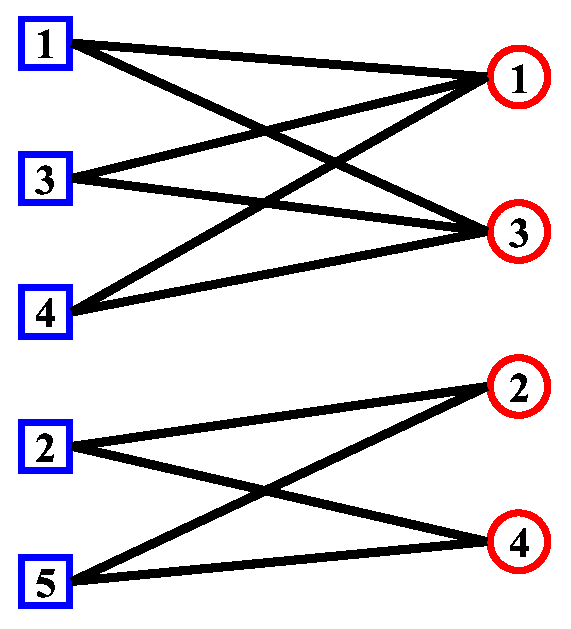
\includegraphics[width=4cm]{Bi_5x4As.eps}}
\put(12,0.8){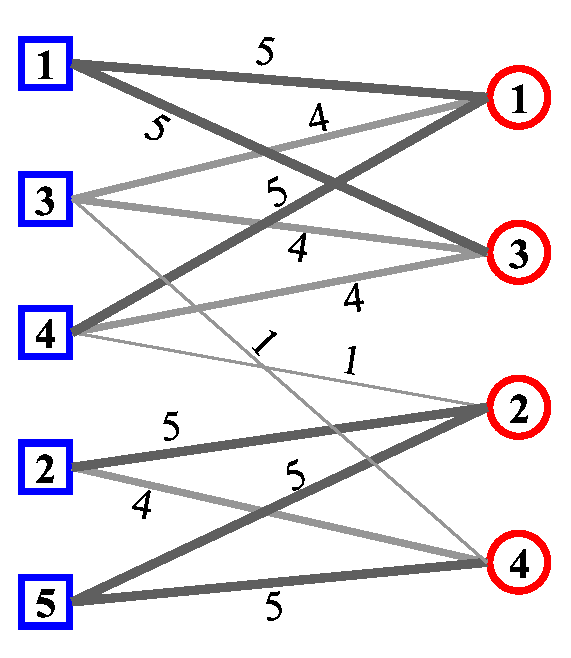
\includegraphics[width=4cm]{Bi_5x4Ws.eps}}
\put(1.8,0){(a)}
\put(7.8,0){(b)}
\put(13.8,0){(c)}
\end{picture}%}
 \caption{対応を表す2部グラフとクラスタリング.
5個の□と4個の○はそれぞれ商品と顧客を表す節である.
(a)商品とそれを買った顧客の対応を枝で表す2部グラフ.
(b) (a)の商品と顧客を並べ替えたもの.
(c)商品と顧客の関連性の強さ(購入数や評価点数など)を
重みとした類似度グラフ.}
\label{fig:Bi_5x4}
\end{center}
\end{figure}



\Section{2部グラフの切断によるデータの同時分類}

{\bf 2部グラフ}(bipartite graph)とは,節がふたつの集合に分かれていて,
一方の集合$M$の節ともう一方の集合$N$の節の間にだけ枝があるようなグラフである.
図\ref{fig:Bi_5x4}のように,
2部グラフは{\bf 対応}(correspondence)を表しており,
その対応次第で,ふたつの集合$M$と$N$の要素を
それぞれ同時にグループ分けできることがある.
そのようなグループ分けは{\bf 共クラスタリング}
(biclustering)%
\footnote{a.k.a. block clustering, co-clustering, or two-mode clustering.}
と呼ばれる.

実際の応用では,要素間の対応の有無ではなく,
関連性の強さで対応が表されていることがある.
例えば,表\ref{tab:stars}のように,
顧客が購入した商品の数や与えた星の数などを参考に,
商品と顧客の関係を調べることになるであろう.
そのような場合は,図\ref{fig:Bi_5x4}(c)のような
{\bf 2部類似度グラフ}(bipartite similarity graph)を作れる.
2部類似度グラフは,集合$M$の要素と集合$N$の要素の
対応を表す枝に重みが与えられている2部グラフである.
なるべく小さな重みの枝を切断して2部類似度グラフを非連結のグラフに
分割することが共クラスタリングであると解釈できる.


\begin{table}[h]
\begin{center}
\caption{関連性の強さで表された対応の例.
顧客と商品の対応を示す値が与えられている.実際の応用では,
顧客が商品を評価した点数かもしれなし,購入数かもしれない.}
\label{tab:stars}
\vspace{\baselineskip}
\begin{tabular}{l|cccc}
        & 顧客1 & 顧客2 & 顧客3 & 顧客4\\
\hline
商品1  & 5 & 0 & 5 & 0 \\
商品2  & 0 & 5 & 0 & 4 \\
商品3  & 4 & 0 & 4 & 1 \\
商品4  & 5 & 1 & 4 & 0 \\
商品5  & 0 & 5 & 0 & 5
\end{tabular}
\end{center}
\end{table}



\Section{2部グラフのスペクトラルクラスタリング}

集合$M$と$N$の要素間の対応を表す$m$対$n$の2部類似度グラフが与えられたとき,
集合$M$と$N$のそれぞれ$k$個のグループに分ける共クラスタリングを実行しよう.
Ncut\cite{Shi00,Yu03})のスペクトラルクラスタリングを
2部類似度グラフに適用すると,次のような計算手順になる.
\begin{enumerate}
\item
与えれれた2部類似度グラフを類似度行列$\mtr W$で表す.
\item
次数行列$\mtr D=\diag(\mtr W\vec 1_{m+n})$を作る.
\item
正規化類似度行列$\mtr S=\mtr D^{-1/2}\mtr W\mtr D^{-1/2}$を作る.
\item
$\mtr S$の$k$個の大きな固有値に属する固有ベクトルを計算し,
固有ベクトルを列に並べた行列
$\mtr X_k=[\vec x^{(1)},\dots,\vec x^{(k)}]\in\mathbb{R}^{(m+n)\times k}$を作る.
\item
$\mtr X_k$の各行を正規化し,ベクトル量子化する.
\end{enumerate}
この手順を更に詳しく見てみよう.


\paragraph{類似度行列の作成}
類似度行列$\mtr W$の第$i$行$j$列要素は第$i$節から第$j$節への
枝の重みである.
$m$対$n$の2部類似度グラフは$m+n$個の節を持つので,
$m+n$次正方の類似度行列で表せる.
$n$個の節を第$m+1,\dots,m+n$節とすると,
$(i,j)\in\{1,\dots,m\}\times\{m+1,\dots,m+n\}$のときだけ
類似度行列の要素$w_{ij}\defas c_{ij}$は非ゼロになり得る.
%ただし,$m$個の節の間に枝は無く,$n$個の節の間にも枝はないので,
%$(i,j)\in\{1,\dots,m\}^2\cup\{m+1,\dots,m+n\}^2$のとき
%隣接行列の要素は$a_{ij}=0$である.
\begin{equation}
\mtr W=\bmatrix{cc}{\mtr O & \mtr C\\ \mtr C^\top & \mtr O}
\label{eq:bipartite affinity matrix}
\end{equation}
類似度行列のブロック行列$\mtr C\in\mathbb{R}^{m\times n}$を
本書では{\bf 長方類似度行列}(rectangular similarity matrix)と呼ぶことにする.
\begin{description}
\item[例:]
図\ref{fig:Bi_5x4}(c)は$m=5$対$n=4$の2部類似度グラフであり,
$m+n=9$個の節を持つ.
商品1から5,顧客1から4を,それぞれ
第1から5節,第6から9節とすると,類似度行列は次のように書ける.
\begin{equation}
\mtr W=\smatrix{\normalsize}{ccccc|cccc}
{
0 & 0 & 0 & 0 & 0  &  5 & 0 & 5 & 0\\
0 & 0 & 0 & 0 & 0  &  0 & 5 & 0 & 4\\
0 & 0 & 0 & 0 & 0  &  4 & 0 & 4 & 1\\
0 & 0 & 0 & 0 & 0  &  5 & 1 & 4 & 0\\
0 & 0 & 0 & 0 & 0  &  0 & 5 & 0 & 5\\
\hline
5 & 0 & 4 & 5 & 0  &  0 & 0 & 0 & 0\\
0 & 5 & 0 & 1 & 5  &  0 & 0 & 0 & 0\\
5 & 0 & 4 & 4 & 0  &  0 & 0 & 0 & 0\\
0 & 4 & 1 & 0 & 5  &  0 & 0 & 0 & 0}
=\bmatrix{cc}{\mtr O & \mtr C\\ \mtr C^\top & \mtr O}
%\end{equation}
\qquad\mbox{ただし,}\quad
\mtr C=\smatrix{\normalsize}{cccc}
{
5 & 0 & 5 & 0\\
0 & 5 & 0 & 4\\
4 & 0 & 4 & 1\\
5 & 1 & 4 & 0\\
0 & 5 & 0 & 5}
\label{eq:bipartite affinity matrix 5x4}
\end{equation}
このように,2部類似度グラフの類似度行列$\mtr W$は,
対角ブロックにゼロ行列,
非対角ブロックに$\mtr C$と$\mtr C^\top$を持つ.
この長方類似度行列$\mtr C$は表\ref{tab:stars}そのものである.
\end{description}

%Ncut\cite{Shi00,Yu03})のスペクトラルクラスタリングでは,
%正規化類似度行列$\mtr S=\mtr D^{-1/2}\mtr W\mtr D^{-1/2}$の
%$k$個の大きな固有値に属する固有ベクトルを列に並べた行列
%$\mtr X_k=[\vec x_1,\dots,\vec x_k]\in\mathbb{R}^{n\times k}$から
%$k$個のクラスタを求める.
%ここで,

\paragraph{次数行列の作成}
$\mtr D=\diag(\mtr W\vec 1_{m+n})$は$\mtr W$の
行和
\begin{equation}
d_{i}=\sum_{j=1}^{m+n}w_{ij}=\left\{
\begin{array}{cll}
\displaystyle\sum_{j=1}^n c_{ij} & \mbox{if $1\leq i\leq m$} & \mbox{($\mtr C$の行和$\mtr C\vec 1_n$)}\\
\displaystyle\sum_{j=1}^m c_{ji} & \mbox{if $m+1\leq i\leq m+n$} & \mbox{($\mtr C$の列和$\mtr C^\top\vec 1_m$)}
\end{array}
\right.
\label{eq:degrees}
\end{equation}
からなる対角行列である.
また,$\mtr D^{-1/2}$も$1/\sqrt{d_i}$からなる対角行列である.
\begin{description}
\item[例:]
式(\ref{eq:bipartite affinity matrix 5x4})の類似度行列から得られる
次数行列$\mtr D$の対角要素は
\begin{eqnarray*}
 \mtr W\vec 1_9&=&[5+5,5+4,4+4+1,5+1+4,5+5,\;\;5+4+5,5+1+5,5+4+4,4+1+5]^\top\\
&=&[10,9,9,10,10,\;14,11,13,10]^\top
\end{eqnarray*}
である.
% The first $m=5$ entries and the following $n=4$ entries are
% the row and column sums of $\mtr C$.
初めの$m=5$個の要素は$\mtr C$の行和,
残りの$n=4$個の要素は$\mtr C$の列和であることがわかる.
\end{description}
%その対角要素の平方根の逆数からなる$\mtr D^{-1/2}$も対角行列である.
%ゆえに,
\paragraph{正規化類似度行列の作成}
正規化類似度行列$\mtr S$の第$i$行$j$列要素は
\[
 s_{ij}=\frac{w_{ij}}{\sqrt{d_id_j}}
\]
であり,式(\ref{eq:bipartite affinity matrix})と同様に
対角ブロックにゼロ行列を持っている.
式(\ref{eq:degrees})のように,$d_{i}$は$\mtr C$の行和と列和からなるので,
正規化類似度行列$\mtr S$は次のように書ける.
\begin{equation}
 \mtr S=\bmatrix{cc}{\mtr O & \mtr Z\\ \mtr Z^\top & \mtr O}
%\end{equation}
\qquad\mbox{ただし,}\quad
\mtr Z=\mtr D_2^{-1/2}\mtr C\mtr D_1^{-1/2},\quad
\mtr D_2=\diag(\mtr C\vec 1_n),\quad
\mtr D_1=\diag(\mtr C^\top\vec 1_m)
\label{eq:normalized affinity matrix}
\end{equation}


\paragraph{固有ベクトルの計算}
式(\ref{eq:normalized affinity matrix})のように,
$\mtr S$はブロック状の$m+n$次正方行列なので,
$m+n$次元の固有ベクトルを持つ.
この固有ベクトルを,
$m$次元ベクトル$\vec u\in\mathbb{R}^m$と
$n$次元ベクトル$\vec v\in\mathbb{R}^n$の連結と見なして
$\vec x=[\vec u^\top\,\vec v^\top]^\top$と置くと,
\begin{eqnarray*}
 \mtr S\vec x&=&\lambda\vec x\\
\bmatrix{cc}{\mtr O & \mtr Z\\ \mtr Z^\top & \mtr O}
\bmatrix{c}{\vec u\\ \vec v}
&=&
\bmatrix{c}{\lambda\vec u\\ \lambda\vec v}
\end{eqnarray*}
\begin{equation}
\therefore\quad
\mtr Z\vec v=\lambda\vec u,\qquad
\mtr Z^\top\vec u=\lambda\vec v
\label{eq:two eigen}
\end{equation}
$\vec u$または$\vec v$を消去すると,次式を得る.
\begin{equation}
 \mtr Z\mtr Z^\top\vec u=\lambda^2\vec u,\quad
\mtr Z^\top\mtr Z\vec v=\lambda^2\vec v
\label{eq:uv}
\end{equation}
%ただし,$\kappa=\lambda^2$である.
すなわち,
$\mtr S$の固有ベクトル$\vec x$を構成する
$\vec u$および$\vec v$は,それぞれ対称行列
$\mtr Z\mtr Z^\top\in\mathbb{R}^{m\times m}$および
$\mtr Z^\top\mtr Z\in\mathbb{R}^{n\times n}$の
固有ベクトルに他ならない.



\paragraph{ふたつの集合のクラスタリング}

$\mtr S$の$k$個の大きな固有値に属する
固有ベクトル$\vec x^{(1)},\dots,\vec x^{(k)}$を列に並べて,
行列$\mtr X_k=[\vec x^{(1)},\dots,\vec x^{(k)}]$を作成する.
行列$\mtr X_k$の全$m+n$行を$k$次元空間の$m+n$点と見なすと,
$k$箇所に固まってクラスタが形成されている.
これは,2部グラフの節のふたつの集合$M$と$N$の要素が
まとめて$k$個のクラスタに分類されたものである.
集合$M$の要素も$N$の要素も$k$個のクラスタに分けられており,
$M$のクラスタと$N$のクラスタの対応も知ることができる.

%2部グラフの一方の集合$M$をグループ分けするクラスタリングには,
%$\mtr X_k$の第1行から第$m$行までの部分行列を使う.
%同様に,集合$N$のクラスタリングには
%$\mtr X_k$の第$m+1$行から第$m+n$行までの部分行列を使う.

\begin{description}
\item[例:]
式(\ref{eq:bipartite affinity matrix 5x4}),(\ref{eq:normalized affinity matrix})
から得られる正規化類似度行列の固有値は
\[
1.00,\;0.92,\;0.12,\;0.03,\;0.00,\;-0.03,\;-0.12,\;-0.92,\;-1.00
\]
である.明らかに大きな固有値がふたつ存在し,
それらに属する固有ベクトルを列に並べると
\begin{equation}
\mtr X_2=[\vec x^{(1)},\vec x^{(2)}]=
\smatrix{\small}{rr}{
    0.32 &   0.31\\
    0.31 &  -0.38\\
    0.31 &   0.22\\
    0.32 &   0.24\\
    0.32 &  -0.40\\
    0.38 &   0.34\\
    0.34 &  -0.39\\
    0.37 &   0.33\\
    0.32 &  -0.36}
\quad\mbox{各行を正規化すると}\quad
\bar{\mtr X}_2
=\smatrix{\small}{rr}{
    0.72 &   0.69\\
    0.63 &  -0.78\\
    0.81 &   0.58\\
    0.80 &   0.59\\
    0.63 &  -0.78\\
    0.75 &   0.66\\
    0.66 &  -0.75\\
    0.75 &   0.66\\
    0.66 &  -0.75}
\end{equation}
という行列を作れる.
各行を$k=2$次元空間の点のデータと見なし,
第1行から第5行の$m=5$点を集合$M$の要素,
第6行から第9行の$n=4$点を集合$N$の要素としてプロットすると,
図\ref{fig:biNcut5vs4}のように2箇所に固まったクラスタが
形成されていることがわかる.
%ベクトル量子化して容易にクラスタを特定できる.
\end{description}
\begin{figure}[h]
\setlength{\unitlength}{1cm}
\begin{center}
%\fbox{
\begin{picture}(6,5)
\put(0,0){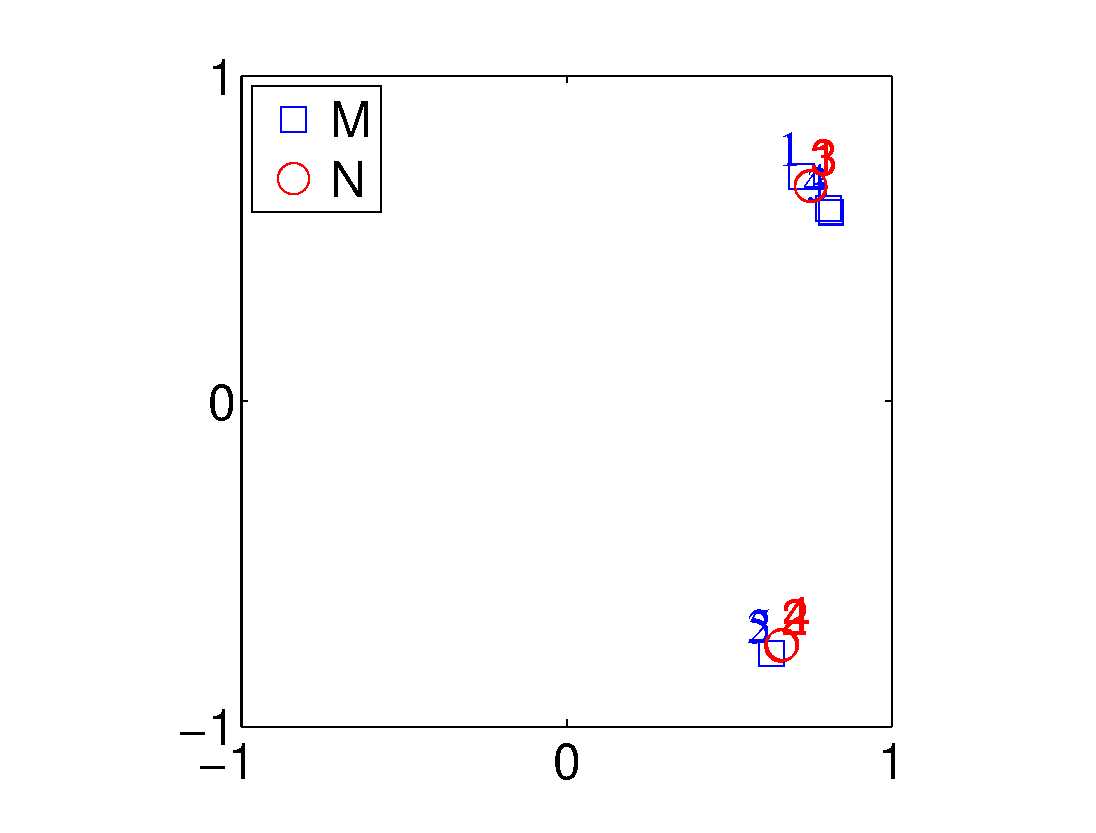
\includegraphics[width=6cm]{biNcut5vs4.eps}}
\end{picture}%}
 \caption{$\bar{\mtr X}_2$の5行が2次元空間でふたつの密なクラスタを呈す.
右上のクラスタは集合$M$の$\{1,3,4\}$と集合$N$の$\{1,3\}$からなる.
右下のクラスタは集合$M$の$\{2,5\}$と集合$N$の$\{2,4\}$からなる.
}
\label{fig:biNcut5vs4}
\end{center}
\end{figure}



\Section{特異値分解}

$\mtr Z$のランクを$r\defas\rank\mtr Z$とし,
%$\rank\mtr Z\mtr Z^\top=\rank\mtr Z^\top\mtr Z=r$が
%成り立つ(演習問題\ref{ex:rankZZ}).
%式(\ref{eq:uv})から,
%$r$個の非ゼロ固有値$\lambda_j^2$と
%これに属する$r$本の固有ベクトル$\vec u^{(j)}$と$\vec v^{(j)}$ ($j=1,\dots,r$)
%が存在する(演習問題\ref{ex:nonzero eigs}).
式(\ref{eq:uv})の非ゼロ固有値$\lambda_j^2$に属する
固有ベクトル$\vec u^{(j)}$と$\vec v^{(j)}$ ($j=1,\dots,r$)は
単位ベクトルであるとする.
対称行列の固有ベクトルは互いに直交するので,
\begin{equation}
\mtr U_r\defas[\vec u^{(1)},\dots,\vec u^{(r)}]\;\in\mathbb{R}^{m\times r}, \qquad
\mtr V_r\defas[\vec v^{(1)},\dots,\vec v^{(r)}]\;\in\mathbb{R}^{n\times r}
\label{eq:matrices of singular vectors}
\end{equation}
という行列を定義すると,
\begin{equation}
 \mtr U_r^\top\mtr U_r=\mtr V_r^\top\mtr V_r=\mtr I\in\mathbb{R}^{r\times r}
\label{eq:orthonormality}
\end{equation}
が成立する.
さらに,
固有値からなる対角行列を$\mtr K_r\defas\diag(\lambda_1,\dots,\lambda_r)$とすると,
式(\ref{eq:two eigen}),(\ref{eq:matrices of singular vectors}),(\ref{eq:orthonormality})から,
次式が導出される(演習問題\ref{ex:UZV}).
\begin{equation}
\mtr Z\mtr V_r=\mtr U_r\mtr K_r,\qquad
%\mtr Z^\top\mtr U=\mtr V\mtr K,\qquad
\therefore\quad
\mtr U_r^\top\mtr Z\mtr V_r=\mtr K_r
\label{eq:SVDr}
\end{equation}

%$\mtr U_r$と$\mtr V_r$はそれぞれ
%$m$次元実空間$\mathbb{R}^m$と
%$n$次元実空間$\mathbb{R}^n$における
%正規直交基底のうち$r$本の基底ベクトルであると見なせる.
$\mtr U_r$は$m$次元実空間$\mathbb{R}^m$の
正規直交基底のうち$r$本の基底ベクトルを並べた行列であると見なせる.
$\mtr V_r$についても同様である.
ゆえに,それぞれ残りの$m-r$本,$n-r$本の
基底ベクトルを追加した行列
$\mtr U\in\mathbb{R}^{m\times m}$と
$\mtr V\in\mathbb{R}^{n\times n}$を作成できる.
これら$\mtr U$と$\mtr V$は直交行列であり,
\begin{equation}
\mtr U^\top\mtr U=\mtr I\in\mathbb{R}^{m\times m},\qquad
\mtr V^\top\mtr V=\mtr I\in\mathbb{R}^{n\times n}
\label{eq:full orthonormality}
\end{equation}
を満たす.
ゆえに,
\begin{equation}
 \mtr Z=\mtr U\mtr K\mtr V^\top=\mtr U_r\mtr K_r\mtr V_r^\top
\label{eq:SVD}
\end{equation}
が成立する.
これは,行列$\mtr Z$の{\bf 特異値分解}(singular value decomposition; SVD)
と呼ばれている.
$\lambda_1,\dots,\lambda_r$は$\mtr Z$の特異値と呼ばれる.
また,$\vec u^{(1)},\dots,\vec u^{(r)}$と
$\vec v^{(1)},\dots,\vec v^{(r)}$は,それぞれ
$\mtr Z$の左特異ベクトル,右特異ベクトルと呼ばれる.




特異値分解を用いると,Ncutによる共クラスタリングは
アルゴリズム\ref{alg:biNcut}のような簡潔な手順になる.
\begin{algorithm}[t]
\caption{Ncutによる共クラスタリング}
\label{alg:biNcut}
\begin{algorithmic}[1]
\REQUIRE
クラスタ数$k$,\\
  $m$個の項目と$n$個の項目の間の関連性の強さを要素とする
長方類似度行列$\mtr C\in\mathbb{R}^{m\times n}$;
% relationships between pairwise items in two sets $M$ and $N$.
\ENSURE クラスタの集合$\mathcal{M}=\{ M_1,\dots,M_k \}$,$\mathcal{N}=\{ N_1,\dots,N_k \}$\\
  (ただし,$\sum_{l=1}^k|M_l|=m$,$\sum_{l=1}^k|N_l|=n$);
\STATE
行和と列和による次数行列$\mtr D_2=\diag(\mtr C\vec 1_n$と$\mtr D_1=\diag(\mtr C^\top\vec 1_m)$を計算する;
%\STATE
%正規化した長方類似度行列$\mtr Z=\mtr D_2^{-1/2}\mtr C\mtr D_1^{-1/2}$の
%$k$個の大きな特異値に属する左右の特異ベクトルを列に並べて,
%行列$\mtr U_k=[\vec u^{(1)},\dots,\vec u^{(k)}]\in\mathbb{R}^{m\times k}$と
%$\mtr V_k=[\vec v^{(1)},\dots,\vec v^{(k)}]\in\mathbb{R}^{n\times k}$を作る;
%\STATE
%$\mtr U_k$と$\mtr V_k$を結合して$\mtr X_k=\bmatrix{c}{\mtr U_k\\ \mtr V_k}\in\mathbb{R}^{(m+n)\times k}$を作る;
\STATE
正規化した長方類似度行列$\mtr Z=\mtr D_2^{-1/2}\mtr C\mtr D_1^{-1/2}$の
$k$個の大きな特異値に属する左右の特異ベクトル$\vec u^{(l)}$と$\vec v^{(l)}$ ($l=1,\dots,k$)を計算する;
\STATE
$\vec u^{(l)}$と$\vec v^{(l)}$を結合して
$\mtr X_k=\bmatrix{ccc}{\vec u^{(1)} & \cdots & \vec u^{(k)}\\ \vec v^{(1)} & \cdots & \vec v^{(k)}}\in\mathbb{R}^{(m+n)\times k}$を作る;
\STATE
$\mtr X_k$の各行ベクトルを正規化する;
\STATE
% quantize each row vector of $\mtr X_k$ into $k$ bins
$\mtr X_k$の各行を$k$個のビンにベクトル量子化して$\vec y\in[k]^{m+n}$を作る:
典型的には,$\mtr X_k$の$m+n$本の
行ベクトルを$k$平均クラスタリングする;
\STATE
$y_i=l$ ($i=1,\dots,m$) ならば項目$i$を$M_l$に所属させる.
\STATE
$y_{m+j}=l$ ($j=1,\dots,n$) ならば項目$j$を$N_l$に所属させる.
\end{algorithmic}
\end{algorithm}



\iffalse
まず,2部グラフの隣接行列から作ったラプラシアン行列の固有ベクトルが
クラスタ指示ベクトルになっていることを確認しよう.
$m$対$n$の2部グラフは$m+n$個の節を持ち,$m+n$次正方の隣接行列で表せる.
$n$個の節を第$m+1,\dots,m+n$節とすると,
$(i,j)\in\{1,\dots,m\}\times\{m+1,\dots,m+n\}$のときだけ
隣接行列の要素$a_{ij}\defas b_{ij}$は非ゼロになり得る.
%ただし,$m$個の節の間に枝は無く,$n$個の節の間にも枝はないので,
%$(i,j)\in\{1,\dots,m\}^2\cup\{m+1,\dots,m+n\}^2$のとき
%隣接行列の要素は$a_{ij}=0$である.
例えば,図\ref{fig:Bi_5x4}(a)は$m=5$対$n=4$の2部グラフであり,
$m+n=9$個の節を持つ.
商品1から5,顧客1から4を,それぞれ
節1から5,節6から9とすると,隣接行列は次のように書ける.
\begin{equation}
\mtr A=\smatrix{\normalsize}{ccccc|cccc}
{
0 & 0 & 0 & 0 & 0  &  1 & 0 & 1 & 0\\
0 & 0 & 0 & 0 & 0  &  0 & 1 & 0 & 1\\
0 & 0 & 0 & 0 & 0  &  1 & 0 & 1 & 0\\
0 & 0 & 0 & 0 & 0  &  1 & 0 & 1 & 0\\
0 & 0 & 0 & 0 & 0  &  0 & 1 & 0 & 1\\
\hline
1 & 0 & 1 & 1 & 0  &  0 & 0 & 0 & 0\\
0 & 1 & 0 & 0 & 1  &  0 & 0 & 0 & 0\\
1 & 0 & 1 & 1 & 0  &  0 & 0 & 0 & 0\\
0 & 1 & 0 & 0 & 1  &  0 & 0 & 0 & 0}
=\bmatrix{cc}{\mtr O & \mtr B\\ \mtr B^\top & \mtr O}
%\end{equation}
\qquad\mbox{ただし,}\quad
\mtr B=\smatrix{\normalsize}{cccc}
{
1 & 0 & 1 & 0\\
0 & 1 & 0 & 1\\
1 & 0 & 1 & 0\\
1 & 0 & 1 & 0\\
0 & 1 & 0 & 1}
\end{equation}
\fi




\Section{演習問題}
\begin{enumerate}
\item
\label{ex:UZV}
式(\ref{eq:SVDr})を導出せよ.
また,特異値分解の式(\ref{eq:SVD})を導出せよ.
\end{enumerate}




{\footnotesize
\bibliography{mybib_cls}
}



